%%%%%%%%%%%%%%%%%%%%%%%%%%%%%%%%%%%%%%%%%%%%%%%%%%%%%%%%%%%%%%%%%%%%%%%%%%%
%                                                                         %
%                         PROJECT INTRODUCTION                            %
%                                                                         %
%%%%%%%%%%%%%%%%%%%%%%%%%%%%%%%%%%%%%%%%%%%%%%%%%%%%%%%%%%%%%%%%%%%%%%%%%%%
\chapter{Introduction} 
\label{chap:Intro}
Radiation Portal Monitors (RPMs) are passive radiation detection systems implemented at over a thousand of border crossings, designed to determine if cargo contains any special nuclear material in a safe, nondestructive, and effective manner\cite{kouzes_neutron_2010}. 
However, the current technology used in RPMs for detecting neutrons emitted from special nuclear material use a rapidly diminishing resource, \iso[3]{He}, that cannot be economically replaced. 
The Department of Homeland Security (DHS) continues to fund research (through the Domestic Nuclear Detection Office (DNDO)) for the development of detector systems to detect radioactive material that could potentially be used to cause significant economic loss and loss of life.  
As a result of this research a number of alternative detection systems continue to be investigated with the most viable including: boron trifluoride filled proportional detectors, boron-lined proportional detectors, \iso[6]{Li} loaded scintillation glass fiber detectors, and \iso[6]{Li} plus scintillator-coated wavelength-shifting fiber detectors\cite{pnnl_18471,kouzes_neutron_2010}.  

Neutron detectors often utilize a material with a large cross section for absorption, such as \iso[6]{Li} or \iso[10]{B}.
When these materials absorb a neutron they usually disintegrate to produce ionized reaction products that in turn transfer their kinetic energy to electrons.
In the case of the $\iso[6]{Li}\left(n,\iso[3]{H}\right)\alpha$ reaction, the fission energy is distributed between a triton of energy \SI{2.73}{\mega\eV} and an alpha of energy \SI{2.05}{\mega\eV}.
In a proportional counter such as the \iso[3]{He} based detectors,the energy from the charged particles would ionize a gas, creating a voltage signal.
Scintillator detectors, on which this work is based, utilize the charged particle energy depositions to create electron excitations in the scintillating material which are then harvested by fluors and produce visible light, which is detected with a photomultiplier tube.


\section{Replacement Detector Criteria}
\label{sec:ReplacmentCriteria}
Pacific Northwest National Lab (PNNL) along with the DNDO have developed a set of specifications that that replacement RPMs must meet \cite{kouzes_neutron_2010, kouzes_neutron_1999}. 
In particular 1) an absolute neutron detection efficiency greater than \SI{2.5}{\cps} at \SI{2}{\meter} for a defined moderated  source, 2) an intrinsic gamma-neutron detection efficiency of one in a million, and 3) a gamma absolute rejection ratio for neutrons stating that the performance of the detector should not change by more than 10\% in a \SI{10}{\milli\roetgen\per\hour} gamma field.
These parameters are summarized in \autoref{tab:DHSCritera}.
\begin{table}
  \centering
	\caption{Replacement Portal Monitor Criteria}
	\begin{tabular}{m{8cm} m{6cm} }
	Parameter & Specification \\
	\hline
	\hline
	Absolute neutron detection efficiency & 2.5 cps/ng of \iso[252]{Cf} (in specified test configuration) \\
	Intrinsic gamma-neutron detection efficiency & $ \epsilon_{int,\gamma n}\leq 10^{-6}$ \\
	Gamma absolute rejection ratio for neutrons (GARRn) & $ 0.9 \leq \text{ GARRn }\leq$ 1.1 at 10 mR/h exposure \\
	Cost &  \$ 30,000 per system \\
	\end{tabular}
	\label{tab:DHSCritera}
\end{table}

The absolute neutron detection efficiency $\left (\epsilon_{abs,n} \right )$ is defined as the number of neutron pulses recorded by the detector normalized by the number of neutrons emitted by the source as shown in \autoref{eqn:absn}
\begin{align}
	\label{eqn:absn}
  \epsilon_{abs,n} = \frac{N_{nc}}{N_{ns}}
\end{align}
where \definevar{$N_{nc}$}{neutron count rate} and \definevar{$N_{ns}$}{neutron emission rate from the source}.
DNDO guidelines state that a \iso[252]{Cf} source placed \SI{2}{\meter} from the midpoint of the detector is to be used for the determination of the absolute neutron detection efficiency\cite{pnnl_18471}.
To reduce the gamma ray flux of \iso[252]{Cf} upon a candidate detector the source is shielded by at least \SI{0.5}{\cm} of lead, and the neutron spectrum is then moderated by \SI{2.5}{\cm} of polyethylene\cite{pnnl_18471}.
The intrinsic efficiency, which provides a measure of how sensitive the detector is to incoming radiation, is defined in \eqref{eqn:inteff}.
\begin{align}
  \label{eqn:inteff}
  \epsilon_{int} = \frac{\text{Number Counts Observed}}{\text{Number Quanta for Radiation Crossing Detector}}
\end{align}
The formulation presented in \eqref{eqn:inteff} is then adapted to photons, with the requirement that only one count per a million photons passing through the detector may be registered.
To account for this the subscript $\gamma n$ is added to the intrinsic efficiency \eqref{eqn:inteffNG}
\begin{align}
  \label{eqn:inteffNG}
  \epsilon_{int,\gamma n} &= \frac{P_{pc}}{P_{p\Phi}}
\end{align}
where \definevar{$P_{pc}$}{photon count rate} and \definevar{$P_{p\Phi}$}{photons crossing the detector}.
The intrinsic gamma-neutron detection efficiency is to be measured using either a \iso[192]{Ir}, \iso[137]{Cs}, or \iso[60]{Co} source placed at an appropriate distance so as to produce an exposure rate of \SI{10}{\milli\roetgen\per\hour} at the detector\cite{kouzes_neutron_1999}.
The final detector parameter, the gamma absolute rejection ratio (GARRn), characterizes the detector response in the presence of both a large gamma ray source (\SI{10}{\milli\roetgen\per\hour}) and a \iso[252]{Cf} neutron source (configured as it would be for an absolute neutron detection efficiency measurement).
This criteria, shown in \eqref{eqn:garrn}, implies that the performance of the detector should not change by more than 10\% in a strong gamma field\cite{kouzes_neutron_1999}.
\begin{align}
  \label{eqn:garrn}
  GARRn = \frac{ \epsilon_{abs,\gamma n}}{\epsilon_{abs,n}}
\end{align}

%%%%%%%%%%%%%%%%%%%%%%%%%%%%%%%%%%%%%%%%%%%%%%%%%%%%%%%%%%%%%%%%%%%%%%%%%%%
%                                                                         %
%                       CURRENT TECHNOLOGIES                              %
%                                                                         %
%%%%%%%%%%%%%%%%%%%%%%%%%%%%%%%%%%%%%%%%%%%%%%%%%%%%%%%%%%%%%%%%%%%%%%%%%%%
\section{Current Technologies}
\label{sec:CurrentTechnologies}
Currently a number of alternative technologies are being developed, but two of the most promising detector technologies are boron loaded straw fibers being developed by Proportional Technologies Inc. (Houston, TX) and LiF loaded ZnS(Ag) scintillator paddles being developed by Innovative American Technology (Coconut Creek, FL).
The boron straw tubes meet the count rate criteria with a gamma rejection rate estimated at \num{4e-9} while passing the GARRn \cite{kouzes_boron-lined_2012}.
LiF/ZnS(Ag) is a commercial inorganic scintillator utilizes the alpha from the \iso[6]{Li} neutron capture to active the ZnS doped with silver (ZnS(Ag)). 
LiF/ZnS(Ag) has a high light output per neutron (\num{1.6E5} photons per neutron) with a decay time of approximately \SI{100}{\micro\second} and the maximum emission at \SI{450}{\nm} \cite{carel_w.e_inorganic-scintillator_2001}.
However, this material is opaque and therefore care needs to be taken with the light collection of a large area detector.
Innovative American Technology (IAT) has developed a design of a replacement RPM that utilizes LiF/ZnS(Ag), as shown schematically in \autoref{fig:IATRender} and in \autoref{fig:IATImage}.
Current testing indicates that this detector design will meet the DHS criteria\cite{kouzes_lithium_2010}.
\begin{figure}
  \centering
  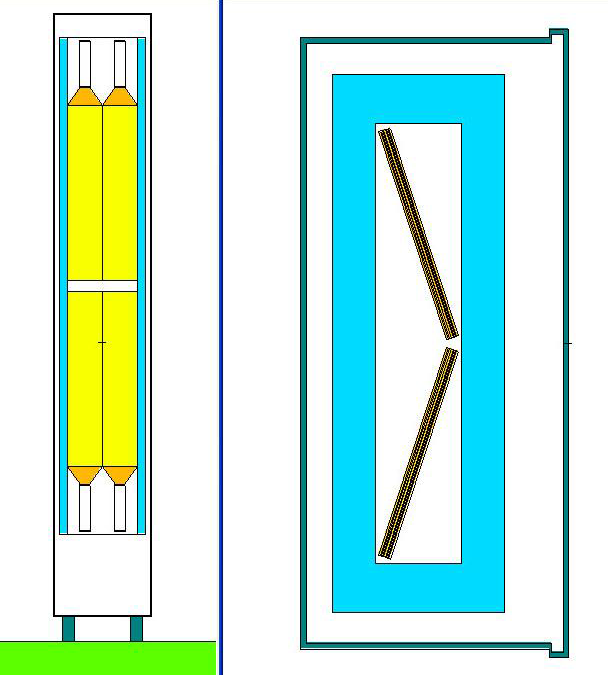
\includegraphics[width=0.5\textwidth]{IATRender}
	\caption[Rendering of IAT Neutron Detector]{Modeled IAT detector that consist of four paddles.  The paddles are angled to expose a larger surface to the neutron flux\cite{pnnl_22228}.}
	\label{fig:IATRender}
\end{figure}
\begin{figure}
  \centering
  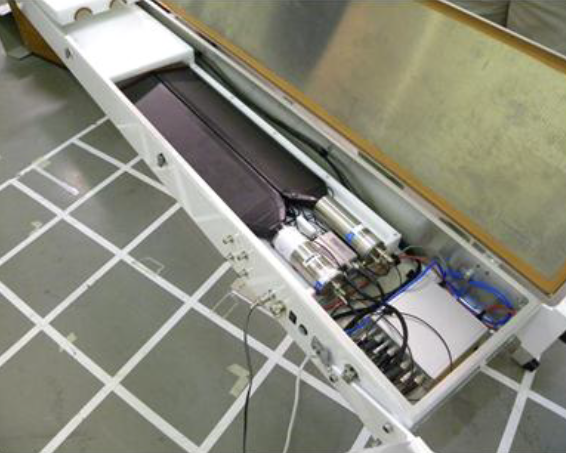
\includegraphics[width=0.75\textwidth]{IATImage}
	\caption[Photograph of IAT Neutron Detector]{Photograph of the developed IAT detector\cite{pnnl_22228}.}
	\label{fig:IATImage}
\end{figure}

%%%%%%%%%%%%%%%%%%%%%%%%%%%%%%%%%%%%%%%%%%%%%%%%%%%%%%%%%%%%%%%%%%%%%%%%%%%
%                                                                         %
%                       DEVELOPED SCINTILLATORS                           %
%                                                                         %
%%%%%%%%%%%%%%%%%%%%%%%%%%%%%%%%%%%%%%%%%%%%%%%%%%%%%%%%%%%%%%%%%%%%%%%%%%%
\section{Developed Scintillators}
\label{sec:DevelopedScintillators}
In addition to the inorganic scintillator LiF/ZnS(Ag), work is being completed at the University of Tennessee to construct thin film polymeric scintillators to be utilized in a layered detector design for replacement RPMs.
These films, either based on polystyrene (PS) or polyethylene naphthalate (PEN), are \iso[6]{LiF} containing polymers projected to be low cost, have high mechanical durability, and meet the detector criteria \cite{Sen_Composites,Mabe201329}.
The developed materials have been characterized for their neutron performance and gamma discrimination abilities, a summary of which (as of May 2013) may be found in \autoref{chap:MeasuredFilmPerfomance}.
%%%%%%%%%%%%%%%%%%%%%%%%%%%%%%%%%%%%%%%%%%%%%%%%%%%%%%%%%%%%%%%%%%%%%%%%%%%
%                                                                         %
%                       OPTIMIZATION INTRODUCTION                         %
%                                                                         %
%%%%%%%%%%%%%%%%%%%%%%%%%%%%%%%%%%%%%%%%%%%%%%%%%%%%%%%%%%%%%%%%%%%%%%%%%%%
\section{Optimization Opportunities}
There exists a need to build predictive modeling capabilities of these detectors in order to optimize the detector performance.
For a particular material and neutron absorber the detector geometry can be optimized to maximize the energy deposited in scintillation material by charged particles relative to the energy deposited by photon interactions. 
This in turn permits one to maximize the recorded neutron interaction rate relative to recorded photon interaction rates by setting a lower level discriminator (LLD) above a threshold associated with energy deposited in the detector by photons.  
As the LLD is increased, the efficiency for detecting neutrons is diminished; however, the intrinsic efficiency for detecting neutrons relative to photons is dramatically increased. 
In addition, as the neutron flux is being moderated and absorbed by the RPM material there exist the opportunity to position the neutron absorber films to maximize the neutron count rate while minimizing the amount of material being used.
Finally, it is essential to ensure that the scintillation light can be collected efficiency.

%%%%%%%%%%%%%%%%%%%%%%%%%%%%%%%%%%%%%%%%%%%%%%%%%%%%%%%%%%%%%%%%%%%%%%%%%%%
%                                                                         %
%                       ORGINAL CONTRIBUTION                              %
%                                                                         %
%%%%%%%%%%%%%%%%%%%%%%%%%%%%%%%%%%%%%%%%%%%%%%%%%%%%%%%%%%%%%%%%%%%%%%%%%%%
\section{Original Contribution}
\label{sec:OrginalContribution}
The design of effective radiation portal monitors is a critical component in detecting and subsequent interdiction of special nuclear material.
Most researchers assume that adequate neutron-gamma discrimination can be achieved by the relatively low mass attenuation coefficient for polymers and taking advantage of the thinness of a detector, but for a common plastic based scintillator the detector would have to be less than \SI{160}{\nm} in order to have an interaction rate less than one in a million.
This work is unique in that the fundamental physics basis of the neutron-gamma discrimination is not attributed to the mass attenuation coefficient but rather to the ranges of the secondary electrons from photon interactions in the material depositing less energy than their neutron counterparts.
Current modeling work in large area neutron detectors focuses either with monolithic plastic slab geometries or with neutronic calculations that do account for light collection and transport.
A layered detector design, while not unique, has not been optimized using a genetic algorithm for which the formulation or the problem is quite natural.
In addition, little modeling work has been completed on the performance of a radiation portal monitor including light transport, which is a large majority of this work.


%%%%%%%%%%%%%%%%%%%%%%%%%%%%%%%%%%%%%%%%%%%%%%%%%%%%%%%%%%%%%%%%%%%%%%%%%%%
%                                                                         %
%                               DOCUMENT LAYOUT                           %
%                                                                         %
%%%%%%%%%%%%%%%%%%%%%%%%%%%%%%%%%%%%%%%%%%%%%%%%%%%%%%%%%%%%%%%%%%%%%%%%%%%
The layout of this document follows the optimization of the design from the detector material to the optimal placement of the material.
\autoref{chap:SecElectron} describes the measurements and simulations preformed in order to determine the the optimal thickness for a single film.
\autoref{chap:GARPMOpt} provides an overview of the various designs that could be considered to utilize the detector material, and then a layered detector design is optimized with the use of a genetic algorithm.
The detector design is finalized in \autoref{chap:LightTransport} where light transport is employed to determine if the detector design would be feasible given a films measured performance.
Finally, \autoref{chap:Conclusions} serves to summarize the various lessons of the detector design.
